\section{Ex1: Poisson Solver with Finite Differences}
\label{sec:fdm}
The first excercise consists of solving the two dimensional Poisson's equation with Finite Differences and utilize the parallel programming paradigm using the Message Passing Interface (\texttt{MPI}) library. We omit specifics here. The exact mathematical description along with the solution strategies are given in \cite{labex1}.
\subsection{Building a parallel version using \texttt{MPI}}
With the help of the sequential Poisson solver, \texttt{SEQ\_Poisson.c}, the build of important tasks of the parallel version is described in this section.  
\subsubsection*{Step 1}
To execute clones of the original code in a number of processes, the following additions are made to the main program of the sequential code.\\

\begin{lstlisting}[style=CStyle]
 MPI_Init(&argc, &argv);
 MPI_Finalize();
\end{lstlisting}
The program was executed twice since two pairs of statements were written to the terminal in comparison to one pair before the modifications. Since we are now running the same program in two different nodes this behavior is expected.

\subsubsection*{Step 4}
Each process wrote to a separate file that does not affect the text displayed. In addition, \texttt{diff} showed no differences between the 2 outputs \texttt{output0.dat} and \texttt{output1.dat}.

\subsubsection*{Step 5}
With the following code incorporated in \texttt{Setup\_Grid()}, only the process with rank 0 reads data from an input file and subsequently broadcasts this data to all processes. Note that the dots represent code already given in the questions.\\
\begin{lstlisting}[style=CStyle]
 if(proc_rank==0){
   .
   .
   .
 }
 MPI_Bcast(&gridsize ,2,MPI_INT ,0,MPI_COMM_WORLD);
 MPI_Bcast(&precision_goal ,1,MPI_DOUBLE ,0,MPI_COMM_WORLD);
 MPI_Bcast(&max_iter ,1,MPI_INT ,0,MPI_COMM_WORLD);

 do {
   if(proc_rank==0)
   ...
   MPI_Bcast(&s,1,MPI_DOUBLE ,0,MPI_COMM_WORLD);
   if(s==3){
     MPI_Bcast(&source_x ,1,MPI_DOUBLE ,0,MPI_COMM_WORLD);
     MPI_Bcast(&source_y ,1,MPI_DOUBLE ,0,MPI_COMM_WORLD);
     MPI_Bcast(&source_val ,1,MPI_DOUBLE ,0,MPI_COMM_WORLD);
     .
     .
     .
   }
 }
 while (n==3);
 if(proc_rank==0) fclose(f); 
\end{lstlisting}
This step demonstrates the use of \texttt{MPI\_Bcast}.
\subsubsection*{Step 6}
This step helps to assign specific tasks to each process. The following are added to \texttt{Setup\_Proc\_grid()}
\begin{lstlisting}[style=CStyle]
 // Retrieve the no of processes
 MPI_Comm_size(MPI_COMM_WORLD ,&P);
 
 //new comm
 MPI_Cart_create(MPI_COMM_WORLD ,2,P_grid,periods,reorder ,&grid_comm);

 // Retrieve new rank and cartesian coordinates of this process
 MPI_Comm_rank(grid_comm ,&proc_rank);
 MPI_Cart_coords(grid_comm ,proc_rank ,2,proc_coord);
 
 //calculate ranks of neighbouring processes
 MPI_Cart_shift(grid_comm ,1,1,&proc_bottom ,&proc_top);
 MPI_Cart_shift(grid_comm ,0,1,&proc_left ,&proc_right);
\end{lstlisting}
\subsubsection*{Step 8}
This step is to setup \texttt{MPI\_Datatypes()} which is a datatype that makes communication convenient, and to perform communication. The following code is used
\begin{lstlisting}[style=CStyle]
 void Exchange_Borders()
 {

  resume_timer();
  Debug("Exchange_Borders",0);
  
  MPI_Sendrecv(&phi[1][dim[Y_DIR]-2],1,border_type[Y_DIR], proc_top,1,
	       &phi[1][0],1,border_type[Y_DIR], proc_bottom, 1,
	       grid_comm, &status);
  
  MPI_Sendrecv(&phi[1][1],1,border_type[Y_DIR],proc_bottom,2,
               &phi[1][dim[Y_DIR]-1],1,border_type[Y_DIR],proc_top,2,
               grid_comm,&status);
  
  MPI_Sendrecv(&phi[1][1],1,border_type[X_DIR],proc_left,3,
               &phi[dim[X_DIR]-1][1],1,border_type[X_DIR],proc_right,3,
               grid_comm,&status);

  MPI_Sendrecv(&phi[dim[X_DIR]-2][1],1,border_type[X_DIR],proc_right,4,
               &phi[0][1],1,border_type[X_DIR],proc_left,4,
               grid_comm,&status);
  stop_timer();
  data_communicated += (2 * dim[X_DIR] + 2 * dim[Y_DIR] - 8);
  
 }
\end{lstlisting}
\newpage
\subsection{Performance Experiments}
This section will describe the results of \emph{experiments} performed on the parallel version of the code described in the previous section. We follow the guidelines given in \cite{labex2}.
\subsubsection*{2.1}
Refering to eq.(1) \&(2) in \cite{labex2}, the grid point is updated as,
\begin{equation}
  c_{i,j}^{n} = \frac{\phi_{i-1,j}^{n}+\phi_{i+1,j}^{n}+\phi_{i,j-1}^{n}+\phi_{i,j+1}^{n} - h^{2}S_{i,j}}{4}-\phi_{i,j}
\end{equation}
\begin{equation}
  \phi_{i,j}^{n+1} = \phi_{i,j}^{n} + \omega c_{i,j}^{n}
\end{equation}
We return to the discussion of an optimal relaxation $\omega$ in the next step. 
Implementation of the algorithmic improvement can be found in the \texttt{Do\_Step()} routine in \texttt{MPI\_Poisson.c}. Here we show the corresponding snippet implementing the above.
\begin{lstlisting}[style=CStyle]
 old_phi = phi[x][y];
 c = (phi[x + 1][y] + phi[x - 1][y] +
 phi[x][y + 1] + phi[x][y - 1]) * 0.25;
 phi[x][y] = (1.0 - w)*old_phi + w*c;
\end{lstlisting}
\subsubsection*{2.2}
After implementing the improvement, 10 tests were performed to compare different values for the relaxation parameter $\omega$. The results are summarized in table. From this data we concluded that 1.934 is the optimal value for the relaxation parameter, accomplishing almost 19 times less iterations than the original with $\omega$ equal to one.
\begin{table*}[h]
\centering
\begin{tabular}{llll}
  \hline
  $\omega$ & Wtime (s) & n    & Reduction   \\
  \hline
  1     & 0.194709  & 2355 & 1           \\
  1.9   & 0.041364  & 220  & 10.70 \\
  1.91  & 0.037918  & 194  & 12.13 \\
  1.92  & 0.0369    & 165  & 14.27 \\
  1.93  & 0.032486  & 131  & 17.97 \\
  \textbf{1.934} & \textbf{0.032996}  & \textbf{125} & \textbf{18.84}  \\
  1.936 & 0.032805  & 130  & 18.11 \\
  1.94  & 0.033853  & 142  & 16.58 \\
  1.96  & 0.03741   & 206  & 11.43 \\
  1.98  & 0.059543  & 419  & 5.62
\end{tabular}
\caption{Time, number of iterations obtained and respective iteration reduction for different $\omega$ values. The topology used was pt:441 with g:100x100}
\label{tab:omega}
\end{table*}

\subsubsection*{2.3}
The goal of this exercise is to investigate the scaling behavior of the code with a fixed relaxation parameter. To accomplish that analysis several runs were measured with various grid sizes. In addition different slices were also tested.
\begin{table*}[]
\centering
\begin{tabular}{@{}cllll@{}}
\toprule
                      &      & \multicolumn{2}{c}{Wtime(s)} &         \\ \midrule
g                     & n    & pt: 441       & pt:422       & Speedup \\ \midrule
\multirow{4}{*}{200}  & 50   & 0.036         & 0.019        & 1.89    \\ \cmidrule(l){2-5} 
                      & 100  & 0.052         & 0.038        & 1.37    \\ \cmidrule(l){2-5} 
                      & 200  & 0.081         & 0.064        & 1.27    \\ \cmidrule(l){2-5} 
                      & 300  & 0.11          & 0.089        & 1.24    \\ \midrule
\multirow{4}{*}{400}  & 100  & 0.123         & 0.108        & 1.14    \\ \cmidrule(l){2-5} 
                      & 300  & 0.299         & 0.286        & 1.05    \\ \cmidrule(l){2-5} 
                      & 500  & 0.473         & 0.462        & 1.02    \\ \cmidrule(l){2-5} 
                      & 1000 & 0.862         & 0.854        & 1.01    \\ \midrule
\multirow{5}{*}{800}  & 100  & 0.371         & 0.364        & 1.02    \\ \cmidrule(l){2-5} 
                      & 300  & 0.979         & 0.965        & 1.01    \\ \cmidrule(l){2-5} 
                      & 500  & 1.493         & 1.486        & 1.00    \\ \cmidrule(l){2-5} 
                      & 1000 & 2.787         & 2.777        & 1.00    \\ \cmidrule(l){2-5} 
                      & 2000 & 5.332         & 5.36         & 0.99    \\ \midrule
\multirow{5}{*}{2000} & 100  & 1.81          & 1.786        & 1.01    \\ \cmidrule(l){2-5} 
                      & 300  & 4.985         & 5            & 1.00    \\ \cmidrule(l){2-5} 
                      & 500  & 8.36          & 8.145        & 1.03    \\ \cmidrule(l){2-5} 
                      & 1000 & 16.162        & 16.149       & 1.00    \\ \cmidrule(l){2-5} 
                      & 2000 & 31.886        & 32.142       & 0.99    \\ \midrule
\multirow{5}{*}{3500} & 100  & 5.144         & 5.071        & 1.01    \\ \cmidrule(l){2-5} 
                      & 300  & 14.766        & 14.912       & 0.99    \\ \cmidrule(l){2-5} 
                      & 500  & 24.699        & 24.585       & 1.00    \\ \cmidrule(l){2-5} 
                      & 1000 & 48.828        & 49.286       & 0.99    \\ \cmidrule(l){2-5} 
                      & 2000 & 97.911        & 98.351       & 1.00    \\ \bottomrule
\end{tabular}
\caption{The maximum time for different grid sizes and different slicing arrangements. The number of iterations for each run was fixed to enable a more accurate comparison.}
\label{tab:topology}
\end{table*}
The results of the aforementioned experiment are shown in table \ref{tab:topology}. As one can obverse the different domain partitions have little impact in the overall performance of the program (speedup in the table measures ratio of pt:422 wrt pt:441), even as the grid size increases.
As explained in \cite{labex2} the (average) time t per iteration n
can be parametrized as follows,
\[
  t(n) = \alpha + \beta n
\]

where $ \alpha $ and $ \beta $ are constants that are determined by running the parallel program for fixed number of iterations. Table \ref{tab:linear-fit} describes the constants determined for the same processor topologies and grid sizes as defined in table \ref{tab:linear-fit}

\begin{table*}[]
\centering
\begin{tabular}{@{}lllll@{}}
  \hline
  & \multicolumn{2}{l}{pt:441}  & \multicolumn{2}{l}{pt:422}   \\
  \hline
  g      & $\beta$        & $\alpha$  & $\beta$    & $\alpha$ \\
  \hline
  200  & 0.0002946 & 0.0219 & 0.0003 & 0.0079 \\
  400  & 0.0008    & 0.0508 & 0.0008 & 0.0355 \\
  800  & 0.0026    & 0.1721 & 0.0026 & 0.1548 \\
  2000 & 0.0158    & 0.3079 & 0.0160 & 0.1837 \\
  3500 & 0.0488    & 0.1847 & 0.0491 & 0.1367 \\
\end{tabular}
\caption{Using least-squares method we estimated $\alpha$ and $\beta$ as defined above. The dataset adopted for this computation is present in Table}
\label{tab:linear-fit}
\end{table*}
In order to improve the quality of this an estimation a thorougher study
should be performed with more runs. In addition considering other (non-
linear) parametrization functions, e.g. exponential, may also yield interesting
results.

\subsubsection*{2.4}
Based on the results from the previous question it is expected that the
division of the domains does not result is significantly different running times.
Thus the choice can be arbitrary.

\subsubsection*{2.5}
For this, we explore the convergence criteria (monitor the no. of iterations) for various problem sizes. The file input.dat is altered so as to perform computations for various grid sizes. The results can be summarized by the following table and the plot below.
\begin{table}[h!]
  \centering
  \begin{tabular}{|c|c c c c|}
    \hline
    g & 200 & 300 & 400  & 500  \\
    \hline
    n & 382 & 771 & 1206 & 1664 \\	
    \hline	
  \end{tabular}
  \caption{No. of iterations for various grid sizes ($\omega = 1.95$).}
  \label{n}
\end{table}

\begin{figure}[ht]
  \centering
  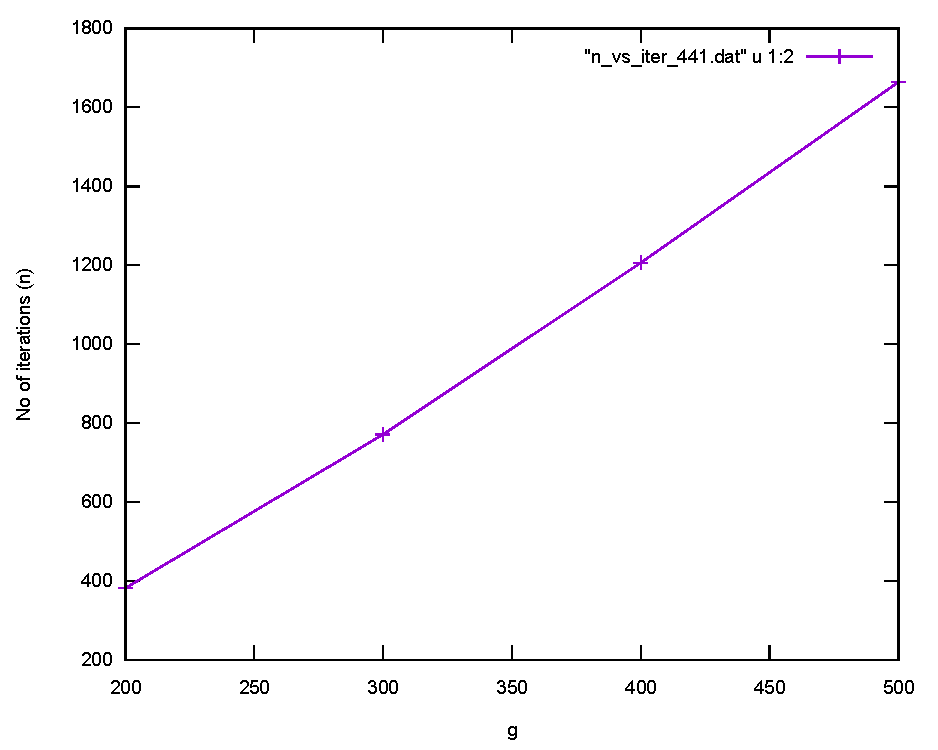
\includegraphics[scale=0.75]{n_vs_iter_441.pdf}
  \caption{\label{fig:n_vs_iter}  g vs n}
\end{figure}

Figure \ref{fig:n_vs_iter} illustrates that as the Problem (grid) size increases, the Number of iterations needed to attain convergence also increases. Computations are done for a topology $4 \times 1$ (pt:441).


\subsubsection*{2.6}
For this, the behaviour is monitored as a function of iteration number. The number ofiterations considered in the x-axis and the magnitude of the error is taken in the y-axis.An optimal $\omega$ of 1.934 was chosen. As expected (also in the plot \ref{fig:}), the error seems to decrease well enough indicating that, with the implementation of Gauss-Seidel with SOR with Red-Black results in earlier convergence than the normal Gauss-Seidel.
\begin{figure}[h]
  \centering
  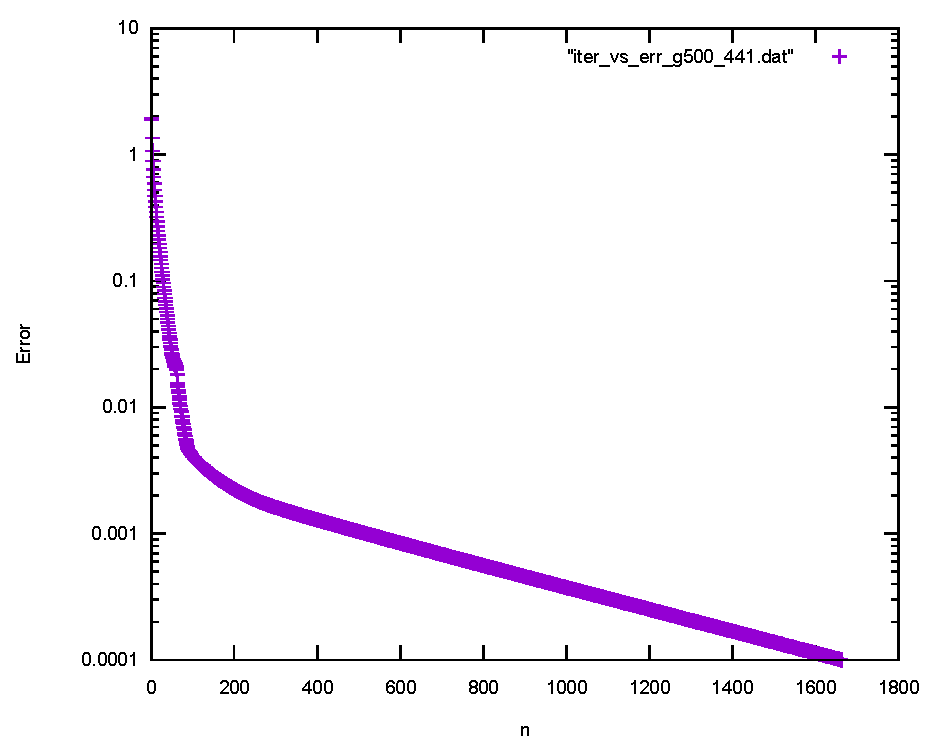
\includegraphics[scale=0.75]{n_vs_err_441_g500.pdf}
  \caption{\label{fig:n_vs_err}  n vs Error for pt:441 and g=500}
\end{figure}
\subsubsection*{2.7}
In an attempt to reduce communication, the global error is calculated and communicated once in 10 iterations. Table \ref{comm1} shows the maximum execution time for the problem with grid size 100 and a 4 $ \times $ 1 topology when the global error is communicated once in every 1, 10 and 100 iterations. Note that $ k $  is the frequency of global error communication and $ t $ is the maximum execution time. \\
	
\begin{table}[h!]
  \centering
  \begin{tabular}{|c|c c c|}
    \hline
    k & 1 		 	& 10 		& 100  \\
    \hline
    t & 0.044293 	& 0.042382  & 0.045240 \\	
    n & 166			& 171	    & 201 \\
    \hline	
  \end{tabular}
  \caption{Communication reduction 1}
  \label{comm1}
\end{table}

	It is found that the communication time and hence the maximum execution time does reduce for a frequency of 10 iterations. However, for a frequency of 100 iterations, the reduction in communication time is superseded by the increase in the number of total iterations needed for convergence. Thus, the total execution time for k = 100 is higher as seen in table \ref{comm1}. The following code is added to the function Solve() for this experiment. \\
	
\begin{lstlisting}[style=CStyle]
if(count%10==0)
MPI_Allreduce(&delta,&global_delta,1,MPI_DOUBLE,MPI_MAX,grid_comm);
\end{lstlisting}

\subsubsection*{2.8}
In another attempt to reduce communication, the red-black sweep of the Gauss-Seidel method is performed more than once between two border exchanges. One red sweep followed by one black sweep is called one full sweep. We perform more than one full sweeps before exchanging the borders. Note that a half sweep means that the borders are exchanged also between red and black sweeps of a full sweep as done in previous exercises. Table \ref{comm2} shows the results obtained. \\
	
\begin{table}[h!]
  \centering
  \begin{tabular}{|c|c c c c|}
    \hline
    k & 1/2 & 1 		 	& 2 		& 3  \\
    \hline
    t & 0.050375 & 0.374343	& 0.679657  & 0.961812 \\	
    n & 166	   & 5000		& 4883	    & 5000 \\
    \hline	
  \end{tabular}
  \caption{Communication reduction 2}
  \label{comm2}
\end{table}

It is evident from the results that the essence of the red-black SOR method is lost by increasing the number of full sweeps between border exchanges. It is also found that despite the solution converging for k=2, the solution is \textit{nan}. Hence it is clear that border exchanges are necessary after every half sweep for convergence. For this experiment, the code in the while loop of the Solve() function is modified as follows. \\
	
\begin{lstlisting}[style=CStyle]
int k=0;

while(k<3)
{
  Debug("Do_Step 0", 0);
  delta1 = Do_Step(0);
  
  Debug("Do_Step 1", 0);
  delta2 = Do_Step(1);
  
  k++;
}   

Exchange_Borders();

delta = max(delta1, delta2);
\end{lstlisting}

\subsubsection*{2.9}
	To sweep only over the points that are to be updated, the inner for loop in the Do$ \textunderscore $Step() function can be modified as shown in the following code. The logic in the inner for loop statement sweeps only over the necessary points thus eliminating the need for a parity check. \\
	
\begin{lstlisting}[style=CStyle]
 for (x = 1; x < dim[X_DIR] - 1; x++)
  for (y = ((x + offset[X_DIR]) % 2)*(1+parity) 
  + !((x + offset[X_DIR]) % 2)*(2-parity); y < dim[Y_DIR] - 1; y+=2)
 if (source[x][y] != 1){
  .
  .
  .
}
\end{lstlisting}
        
For the test problem (pt=441, n=100), the maximum execution reduces from 0.068726 sec to 0.055967 sec by doing the above mentioned modification which ensures that the sweep is only over the points that are supposed to be updated in the red and black iterations. For bigger problem sizes the performance significantly goes up. For the problem with 414 topology and n=1600, maximum execution time reduces from 46.16542 sec to 37.72682 sec.

\subsubsection*{2.10}
For this experiment, the timer is resumed before the \texttt{Exchange\_Borders()} function and stopped right after it as shown in the following code in the \texttt{Do\_Step()} function. 

\begin{lstlisting}[style=CStyle]
 resume_timer();
 Exchange_Borders();
 stop_timer();
\end{lstlisting}
	
	The exchange border time is measured as a function of number of processes and a function of problem size and the results are tabulated in tables \ref{exbor} and \ref{exbor2}.
	
	\begin{table}[h!]
          \centering
          \begin{tabular}{|c|c c c c c c|}
            \hline
            g & 200 & 400 & 800	& 1000  & 2000 & 3500 \\
            \hline
            t & 0.026389 & 0.031386 & 0.080393 & 0.107828 & 0.355372 & 2.019741\\
            \hline	
          \end{tabular}
          \caption{Exchange border time as a function of grid size (pt= 441)}
          \label{exbor}
	\end{table}
        
	\begin{table}[h!]
          \centering
          \begin{tabular}{|c|c c c c c|}
            \hline
            pt & 221 & 441 & 422 &881 &842 \\
            \hline
            t & 0.002634 & 0.04723	& 0.005687 & 0.045410 & 0.047286 \\
            T & 0.028546 & 0.056971 & 0.020753 & 0.061953 & 0.054358 \\
            \hline	
          \end{tabular}
          \caption{Exchange border time as a function of no. of processes (g=100)}
          \label{exbor2}
	\end{table}
It can be seen in table \ref{exbor} that the time spent in exchanging borders is close to the time spent on computations for the following problem: g=200, pt=441. 

\subsubsection*{2.11}
The overhead of the parallel program is given by,
\[
  T_o = pT_p - T_s
\]
	
where $ T_p $ is the parallel execution time and $ T_s $ is the serial execution time. The overhead caused by exchanging borders can be calculated by considering the SOR algorithm with $\omega=1$ and comparing it with the sequential code. For the configurations and grid sizes from exercise 2.3, the overheads are given in the table \ref{overhead}. \\
\begin{table}[h!]
  \centering
  \begin{tabular}{|c|c|c|c|c|c|}
    \hline
    Proc. topology & Grid size & $ T_p $ & $ T_s $ & $ T_o $ \\
    \hline
                   & 200 & 0.195640 & 0.46 & 0.3216 \\
                   & 400 & 0.978629 & 2.86 & 1.0535 \\
    4 $ \times $ 1 & 800 & 2.673317 & 9.65 & 1.0391 \\
                   & 1000 & 5.853645 & 22.54 & 0.8752 \\
                   & 2000 & 22.928791 & 90.24 & 1.4641 \\	
    \hline	
                   & 200 & 0.172482 & 0.46 & 0.2299 \\
                   & 400 & 0.968356 & 2.86 & 1.01 \\
    2 $ \times $ 2 & 800 & 2.87270 & 9.65 & 1.8478 \\
                   & 1000 & 5.924463 & 22.54 & 1.1570 \\
                   & 2000 & 23.025853 & 90.24 & 1.8754 \\	
    \hline
  \end{tabular}
  \caption{Overheads}
  \label{overhead}
\end{table}

\subsubsection*{2.12}
The impact of the communication overhead is limited. Even for large grid sizes halving the amount of data sent is likely to cause, at best, moderate improvements. In addition the maintainability of the code would decrease rapidly as such modifications would hamper readability and comprehension of the code base.
Nonetheless to accommodate this optimization the address of the first point to exchange would have to be calculated differently, taking into account the parity value. Moreover the size of the “jump” between transmittable points would also need to be modified. Such a change would best be done in the \texttt{Setup\_MPI\_Datatypes()} where the custom data types are defined. The greatest advantage would be the 50\% reduction number of points to exchange.



%%% Local Variables:
%%% mode: latex
%%% TeX-master: "report"
%%% End:
